\providecommand{\topdir}{..}
\documentclass[../main.tex]{subfiles}

\newglossaryentry{glos:pibond}{
	name=$\pi$,
	description={A chemical bond between two atoms, due to overlap in $s$ and $p$ orbitals. For example, in Carbon $sp^2$ hybridisation creates $pi$ bonds.}
}
\newglossaryentry{glos:pibondstar}{
	name=$\pi^*$,
	description={An anti-bond version of a $\pi$ bond, due to overlap in $s$ and $p$ orbitals. A higher energy than that of the $\pi$ bond.}
}
\newglossaryentry{glos:sigmabond}{
	name=$\sigma$,
	description={A chemical bond between two atoms, due to overlap in $p$ orbitals perpendicular to the atomic displacement. For example, in Carbon $p^z$ overlap creates $\sigma$ bonds.}
}
\newglossaryentry{glos:sigmabondstar}{
	name=$\sigma^*$,
	description={An anti-bond version of a $\sigma$ bond, due to anti-bonding overlap in $p$ orbitals perpendicular to the atomic displacement. A higher energy than that of the $\sigma$ bond.}
}
\newglossaryentry{glos:hybridisation}{
	name=hybridisation,
	description={The overlap of atomic orbitals that creates bonding and anti-bonding, leading to lower energy (and higher energy) bonding states.}
}
\newglossaryentry{glos:rubbing}{
	name=rubbing,
	description={Mechanical alignment of a film toward a particular orientation, using a brush or some other mechanical device.}
}
\newglossaryentry{glos:blade-coating}{
	name=blade coating,
	description={The use of a blade edge to push and deposit a wavefront of dissolved polymer, to achieve strong film alignment.}
}
\newglossaryentry{glos:stacking-pi}{
	name=$\pi$-stacking,
	description={Stacking in the out-of-plane direction, relative to the 2D molecular plane. The typical miller indices are assigned to the second index, i.e. (0,1,0).}
}
\newglossaryentry{glos:stacking-alkyl}{
	name=alkyl-stacking,
	description={Stacking in the direction of Alkyl side-chains, that is perpendicular to the backbone.}
}
\newglossaryentry{glos:stacking-backbone}{
	name=backbone-stacking,
	description={Stacking along (parallel to) the main chain direction of a polymer.}
}

\begin{document}
	\chapter{Polymers}\label{chap:02-polymers}
		\section{Atomic bonding}\label{sec:ch2-cbonding}
			\Gls{glos:hybridisation} is the creation of new molecular orbitals from the overlap of core electron wavefunctions, and occurs when atoms in a molecule bond with each other. Most molecules are roughly 1D or 2D in nature, but not usually 3D like a crystal. Therefore most molecules bond across two dimensions.
			
			\subsection{Molecular orbitals and Carbon}
				Let's consider carbon, depicted in \cref{fig:ch2-sigma-pi-bonds}. The hybridisation in carbon is called $sp^2$ \gls{glos:hybridisation}. Take the ground-state of carbon: it has two electrons (up \& down spins) in it's $1s$ shell, and 2 electrons in the $1p_{x,y,z}$ shells.
				
				When two carbons overlap, \gls{glos:hybridisation} occurs, creating a \gls{glos:pibond} bond. Because there is an overlap of two atomic orbitals, there are two resulting \textit{molecular} orbitals. These are the bond and anti-bond, in this case \gls{glos:pibond} and \gls{glos:pibondstar}. The anti-bond has a much higher energy level than the bond, and consequently is usually unoccupied.
				However, this isn't the only wavefunction overlap that occurs in carbon, there is also the overlap of the $sp^2$ orbitals which form the strong \gls{glos:sigmabond} and \gls{glos:sigmabondstar} bonds.
				
				\begin{figure}[]
					\centering
					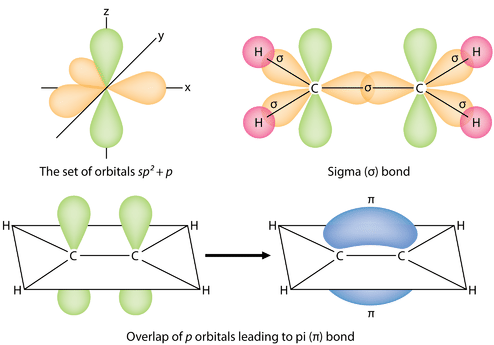
\includegraphics[width=0.6\textwidth]{resources/ch2/ZachWilson-CK12-Sigma-Pi-Bonds}
					\caption{The description of various orbitals and their bonding, including the out-of-plane $p_z$-orbitals (green), the in-plane $sp^2$-orbitals (yellow) caused by the hybridisation of $p_x, p_y, s$ orbitals. The emergence of bonding is also shown, with the overlap of in-plane $sp^2$ orbitals (yellow) to form a strong \gls{glos:sigmabond} bond, and with the overlap of $p_z$-orbitals (green) to form a \gls{glos:pibond} bond (blue) between atoms. Source: Zachary Wilson, CK-12 Foundation \autocite{wilson_924_2016}.}
					\label{fig:ch2-sigma-pi-bonds}
				\end{figure}
			
		\section{Polymer micro-structure and alignment}\label{sec:ch2-alignment}
			\subsection{Stacking}
				Polymer packing is complex, due to the variety of inclusions and degrees of freedom attainable in a film solution. This includes tie-chains and defects.
				
				Typically, for well packed polymers with high degrees of orientation, stacking orientations are as follows:
				\begin{itemize}
					\item \gls{glos:stacking-backbone} is oriented along the direction of the backbone.
					\item \gls{glos:stacking-alkyl} is perpendicular to the backbone, but given the radial freedom of alkyl side-chains, this could be arranged in a variety of ways, or have little net uniformity.
					\item \gls{glos:stacking-pi} is perpendicular to the plane of the molecule, and is primarily related to the parallel alignment of backbones, though will be affected by alkyl behaviour as well.
				\end{itemize}
				Sometimes one type of stacking may exist without the presence of others.
				
			\subsection{Something}
		
			
		\section{Solar Cells}\label{sec:ch2-solar-cells}
			Something else

\ifSubfilesClassLoaded{
	\printbibliography{}
	\printglossaries
}{} % we have no 'else' action
	
\end{document}